\documentclass[11pt]{article}

\usepackage[utf8]{inputenc}
\usepackage[ngerman]{babel}
\usepackage[hyphens]{url}
\usepackage{hyperref}
\usepackage{graphicx}
\usepackage{float}
\usepackage{courier}

\usepackage[normalem]{ulem}

%%%%%%%%%%%%%%%%%%%%%%%%%%%%%%%%%%%%%%%%%%

\title{Dokumentation}
\author{Tanja Noack, Janine Kostka}
\date{\today}

%%%%%%%%%%%%%%%%%%%%%%%%%%%%%%%%%%%%%%%%%%

\begin{document}
	\maketitle  
	\pagebreak
	
	%%%%%%%%%%%%%%%%%%%%%%%%%%%%%%%%%%%%%%%%%%
	
	\tableofcontents
	\pagebreak
	
	%%%%%%%%%%%%%%%%%%%%%%%%%%%%%%%%%%%%%%%%%%
	
	\section{To-Do}
	\begin{itemize}
		\item 
	\end{itemize}
	
	\section{Anforderungen}
	Der Benutzer soll in der App eigene Textschnipsel abspeichern und diese dann mit Tags versehen können. Weiterhin soll der Benutzer nach Snippets suchen können. Dabei sind folgende Methoden möglich: 
	\begin{itemize}
		\item Volltextsuche. Dabei werden die abgespeicherten Texte nach den Worten durchsucht
		\item Tagsuche. Mit Setzen eines '\#' am Anfang der Suche können spezifisch die Tags durchsucht werden
		\item Titelsuche. Mit Setzen eines '@' am Anfang der Suche können spezifisch die Titel durchsucht werden
	\end{itemize}
	
	Der Benutzer soll in der App einstellen können, welche Textschnipsel später auf der Tastatur angezeigt werden können. Diese werden als Favoriten gekennzeichnet. \\
	
	\noindent Für die Tastatur soll eine eigene sogenannte Input Method mittels der bereitgestellten API \sloppy\url{https://developer.android.com/guide/topics/text/creating-input-method.html} geschrieben werden. Statt den einzelnen Tasten sollen dann Inhalte aus der App angezeigt werden, die vom Nutzer selbst festgelegt werden können.\\
	
	Das Projekt besteht somit aus zwei Komponenten:
	\begin{enumerate}
		\item eine App, um die Textschnipsel zu organisieren und die Tastatur zu konfigurieren
		\item eine Tastatur, die ihren Inhalt je nach Einstellung des Benutzers verändert
	\end{enumerate}
	
	\subsection{Funktionale Anforderungen}
	Welche Funktionen sollen dem Nutzer bereitgestellt werden?
	\subsubsection{App}
	\begin{itemize}
		\item Der Benutzer soll eigene Textschnipsel abspeichern, löschen und verändern können
		\item Die Textschnipsel bestehen jeweils aus Text, Name des Schnipsels und einer Liste von Tags
		\item Der Benutzer kann die Textschnipsel in Ordnern organisieren
		\item Der Benutzer kann nach Textschnipseln entweder mittels Volltextsuche, über Tags oder über deren Namen suchen
	\end{itemize}
	
	\subsubsection{Tastatur}
	\begin{itemize}
		\item Anzeige von als Favoriten markierten Textschnipseln als Buttons
		\item Anzeige mit Namen, Einfügen von entsprechend dem Snippet hinterlegten Text
		\item Änderungen werden während der Laufzeit bereits angezeigt
	\end{itemize}
	
	\subsection{Nichtfunktionale Anforderungen}
	\subsection{Anwendungsfälle}
	Nachfolgend einige ausgewählte Anwendungsfälle: \\
	Hier 2-3 Use Case Diagramme mit kurzer Beschreibung einfügen. Das sind sozusagen die angewandten funktionalen Anforderungen, wie sie in einem Szenario während der Nutzung der App auftauchen könnten
	
	
	\section{Implementierung}
	\subsection{Workflow der Dialoge(doofer Titel)}
	Beschreibung der Activites. Welche wird bei welchem Event aufgerufen, z.B. \\
	User befindet sich in der MainActivity -> Tippt auf FAB "+" -> NewSnippetActivity wird aufgerufen \\
	Beschreibung eher aus technischer Sicht im Gegensatz zu den Anwendungsfällen
	
	\subsubsection{App}
	\subsubsection{Tastatur}
	Die angepasste Tastatur ist als eine zusätzliche, normale Android Systemtastatur implementiert worden. Dabei gliedert sich der Aufbau wie folgt: 
	\begin{itemize}
		\item \texttt{xml/keyboard.xml} enthält die Aufteilung der Tastatur, wie diese in \texttt{Keyboard.Row} und \texttt{Keyboard.Key} unterteilt ist
		\item \texttt{xml/method.xml} Festlegen der InputMethod als Systemtastatur
		\item \texttt{layout/keyboard\_view.xml} ist das Layout der Tastatur, welches aufgerufen wird
		\item \texttt{layout/key\_preview.xml} dient der Key-Popup-Funktion, falls ein Key mehrere Symbole ausgeben kann. In unserem Fall wird diese nicht genutzt.
		\item \texttt{SnippetInputService.java} ist die Javaklasse, in welcher die Keyboardfunktionen implementiert wurden, zum Beispiel das Instanzieren des Keyboards, Laden der Snippets aus der Datenbank und entsprechendes Einfügen auf die Knöpfe der Tastatur
	\end{itemize}
	
	
	\subsection{Architektur}
	Welche Frameworks wurden benutzt? Welche Zusammenhänge sind zwischen den Modulen etc.?
	\subsubsection{Tastatur - Extended InputMethodService}
	Für die Tastatur wird der von Android definierte InputMethodService erweitert. \\
	Beschreibung der Klasse SnippetInputService, wie diese Daten aus der DB zieht, die Label und OutputText der Buttons setzt, wie das Layout der Tastatur über die verschiedenen XML-Ressourcen definiert wird.
	
	
	
	\subsubsection{Persistence Layer - Room-Framework}
	Für CRUD-Operationen wird das von Android bereitgestellte Framework genutzt. Dabei wird im Falle der App zusätzlich ein Repository mit ViewModel verwendet. 
	\begin{figure}[H]
		\centering
		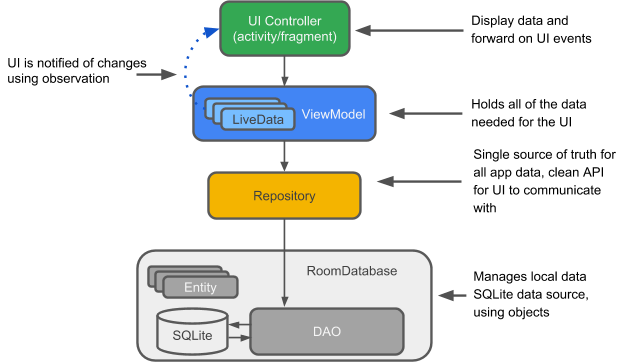
\includegraphics[width=1.0\textwidth]{Konzepte/roomArch.png}
		\caption{Room-Architektur (\sloppy\url{https://codelabs.developers.google.com/codelabs/android-room-with-a-view/})}
		\label{fig:room_arch}
	\end{figure}
	Da für die Tastatur jeweils nur eine Anfrage vom Service aus an die Datenbank gemacht wird.\\
	Es werden 3 Tabellen verwendet, welche folgendes ER-Modell abbilden.
	
	\subsubsection{UI}
	Beschreibung der Activity-Klassen
	
	
	\subsection{Probleme und deren Lösung}
	Falls wir noch Prosa schreiben müssen könnten wir hier auch verworfene Ideen aus den Notizen unten aufführen.
	\subsubsection{Persistenz mit Room-Library}
	Die Textschnipsel sollten in der nativen SQLite-Datenbank gespeichert werden. Wie im Teil der Archtitektur schon beschrieben, werden diese in insgesamt drei Tabellen gespeichert. Diese bilden eine Many-to-many-Relation auf der Datenbankebene ab, da Room nur Annotationen für One-to-Many Relationen bietet. Dementsprechend musste entprechend ein DAO für diese Hilfstabelle erstellt werden. \\
	Schlussendlich war durch die Entscheidung alle Tags nicht csv in einem Attribut pro Element zu speichern dafür gut, dass die Suchfunktion in der App auch in der Lage war nach Tags zu suchen.\\
	Asynchrone Operationen blabla
	\subsubsection{Custom Keyboard}
	Für die Erstellung einer für die Zwecke der App angepassten Tastatur gab es Vorüberlegungen und Ideen, welche später durch mangelnde Möglichkeiten verworfen werden mussten. Dazu zählen unter anderem: 
	\begin{itemize}
		\item Anzeige der (kompletten) Liste an Snippets 
		\item Autovervollständigung: Ab dem Eintippen wird die Liste aktualisiert mit allen Einträgen, die mit der Eingabe beginnen oder sie enthalten
		\item Häufigkeitsanalyse: Anzeige der häufig genutzten Snippets an erster Stelle
		\item Einbinden der Liste der Snippets in Tastatur durch einen extra Menüpunkt: Layout einer normalen Systemtastatur, allerdings mit einem zusätzlichen Button, um auf die Snippets zugreifen zu können
	\end{itemize}
	
	Des Weiteren gab es bei der Implementierung der bestehenden Tastatur Probleme, welche bei der Weiterentwicklung berücksichtigt werden sollten:
	\begin{itemize}
		\item nur outdated Tutorials gefunden
		\item Doku eher unvollständig
		\item Bsp: android:codes akzeptiert laut Doku Strings mit Unicode Charaktern, in der Implementierung werden aber nur Int-Codes akzeptiert
		\item nach einigem Suchen herausgefunden, dass Strings mittels android:keyOutPutText eingefügt werden können. Diese werden nicht über onKey, sonder über onText eingefügt.
	\end{itemize}
	\subsubsection{Definition des Layouts}
	alles durcheinander -> wie hast du das am Ende dann halbwegs geordnet bekommen?
	
	\section{Wer hat was gemacht?}
	Janine alles, Tanja nix.
	Da ichs nie auf die Reihe kriegen werde das persönlich zu sagen, weil ich viel zu awkward für so etwas bin.. es tut mir so Leid, dass ich mich von dir so hab durchs Semester ziehen lassen. Jedes Mal, wenn ich versucht habe etwas anzufangen, ging es einfach nicht, weil mein Kopf sonstwo steckt. Ich bekomme derzeit nichts auf die Reihe außer Kleinigkeiten und selbst bei denen versage ich regelmäßig.
	Danke, dass du es erträgst. Danke, dass du mir hilfst. Danke, dass du mich so durchziehst. 
	
	\section{Erweiterungen}
	Was gibt es, was später noch eingebaut werden könnte?
	\begin{itemize}
		\item Häufigkeitsanalyse: wird viel benutzt -> wird als erstes angezeigt
	\end{itemize}
	
	\section{Notizen}
	\emph{Absprache mit Herrn Schemmert}
	
	Dokumentation:
	\begin{itemize}
		\item Architektur mit einfügen (welche PlugIns, Frameworks, APIs, ... benutzt werden -> Debug Plugin: Stetho (DB auslesen), Room Persistence, API InputMethodService
		\item Klassendiagramm nur wenn sinnvoll -> ist hier nicht wirklich sinnvoll, ist nichts ungewöhnliches oder komplexes dabei
		\item Use Cases wichtig -> Use Cases werden beschrieben + Diagramme
		\item Abspeichern der Schnipsel: Datenbank (SQL lite [relational])? Ein großer JSON-Block? Ein JSON pro Schnipsel? -> SQLite mit 3 Tabellen
	\end{itemize}	
	Aufbau/Entwurf:
	\begin{itemize}
		\item entweder Ordnerstruktur (doof) oder Suche? -> Ordner sind doof, Tags! + Suche
		\item eventuell: Gliederung nach Tags/Themen (dienstlich, privat, ...)/Art (Text, Smiley, ...)/Klassifizierungen/... ne.
		\item App zuerst bauen, weil einfach done.
	\end{itemize}
	
	
	%%%%%%%%%%%%%%%%%%%%%%%%%%%%%%%%%%%%%%%%%%
\end{document}
